\chapter{The Cost of Capital}

\section{Introduction}
\begin{itemize}
    \item Overview of the capital structure decision and its significance in determining the cost of capital for a firm.
    \item Exploration of how to estimate the weighted average cost of capital (WACC) of the firm, building upon the previous session's insights on required rates of return by investors based on systematic risk.
    \item Discussion on the capital asset pricing model (CAPM) and the use of the security market line for pricing the required rate of return of an asset.
    \item Application of these concepts to estimate the firm's cost of capital by assessing the costs associated with equity and debt financing.
    \item Introduction to the calculation of the weighted average cost of capital, combining the costs of equity and debt.
    \item Explanation of how to use the WACC to discount future cash flows in financial analysis and investment decision-making.
\end{itemize}

\section{Reading}
Chapters 10 and 12 of Berk, J.B. \& DeMarzo, P.M (2020). Corporate Finance, 5th Edition. Pearson.

\section{The Cost of Capital}

Consider the pros and cons of debt over equity. This chapter focuses more on the tax differences.

\begin{itemize}
    \item Debt is a business expense so it is tax-deductible. This means that the cost of debt is lower than the cost of equity.
    \item Debt can impose discipline on managers to fulfil interest obligations and avoid bankruptcy.
    \item Debt also has lower cost and quicker access to capital. But accumulating too much of it could make it difficult to raise additional funds.
    \item Excessive debt can influence management behaviour to favour riskier projects over safer ones, even if the latter has a higher net present value.
\end{itemize}

Suppose we have two companies A and B with identical operations, profits before interest in taxes (EBIT) of £1M. Company A has no debt but Company B has taken on a loan with interest expense of £200K. Assume the corporate tax rate is 30\%. We thus have the following financial comparison:

\begin{table}[H]
    \centering
    \caption{Financial Comparison of Company A and Company B}
    \begin{tabular}{@{}lcc@{}}
    \toprule
     & \textbf{Company A (No debt)} & \textbf{Company B (With debt)} \\ 
    \midrule
    EBIT & £1,000,000 & £1,000,000 \\
    Interest expense & 0 & £200,000 \\
    Taxable income & £300,000 & £800,000 \\
    Tax (30\%) & £300,000 & £240,000 \\
    Net income & £700,000 & £560,000 \\
    \bottomrule
    \end{tabular}
\end{table}

At first glance, Company A has a significantly higher net income than Company B, but this is where the tax shield comes into play.\\

\begin{equation}
    \text{Tax Shield} = \text{Interest Expense} \times \text{Tax Rate}
\end{equation}

So in this case, the tax shield for Company B is £200,000 $\times$ 30\% = £60,000. This is the savings in taxes that Company B gets. Even though Company B has a lower net income, it has more cash to distribute to shareholders and bondholders.\\

\subsection{Analytical View of the Firm for Capital Structure}
\begin{figure}[H]
    \centering
    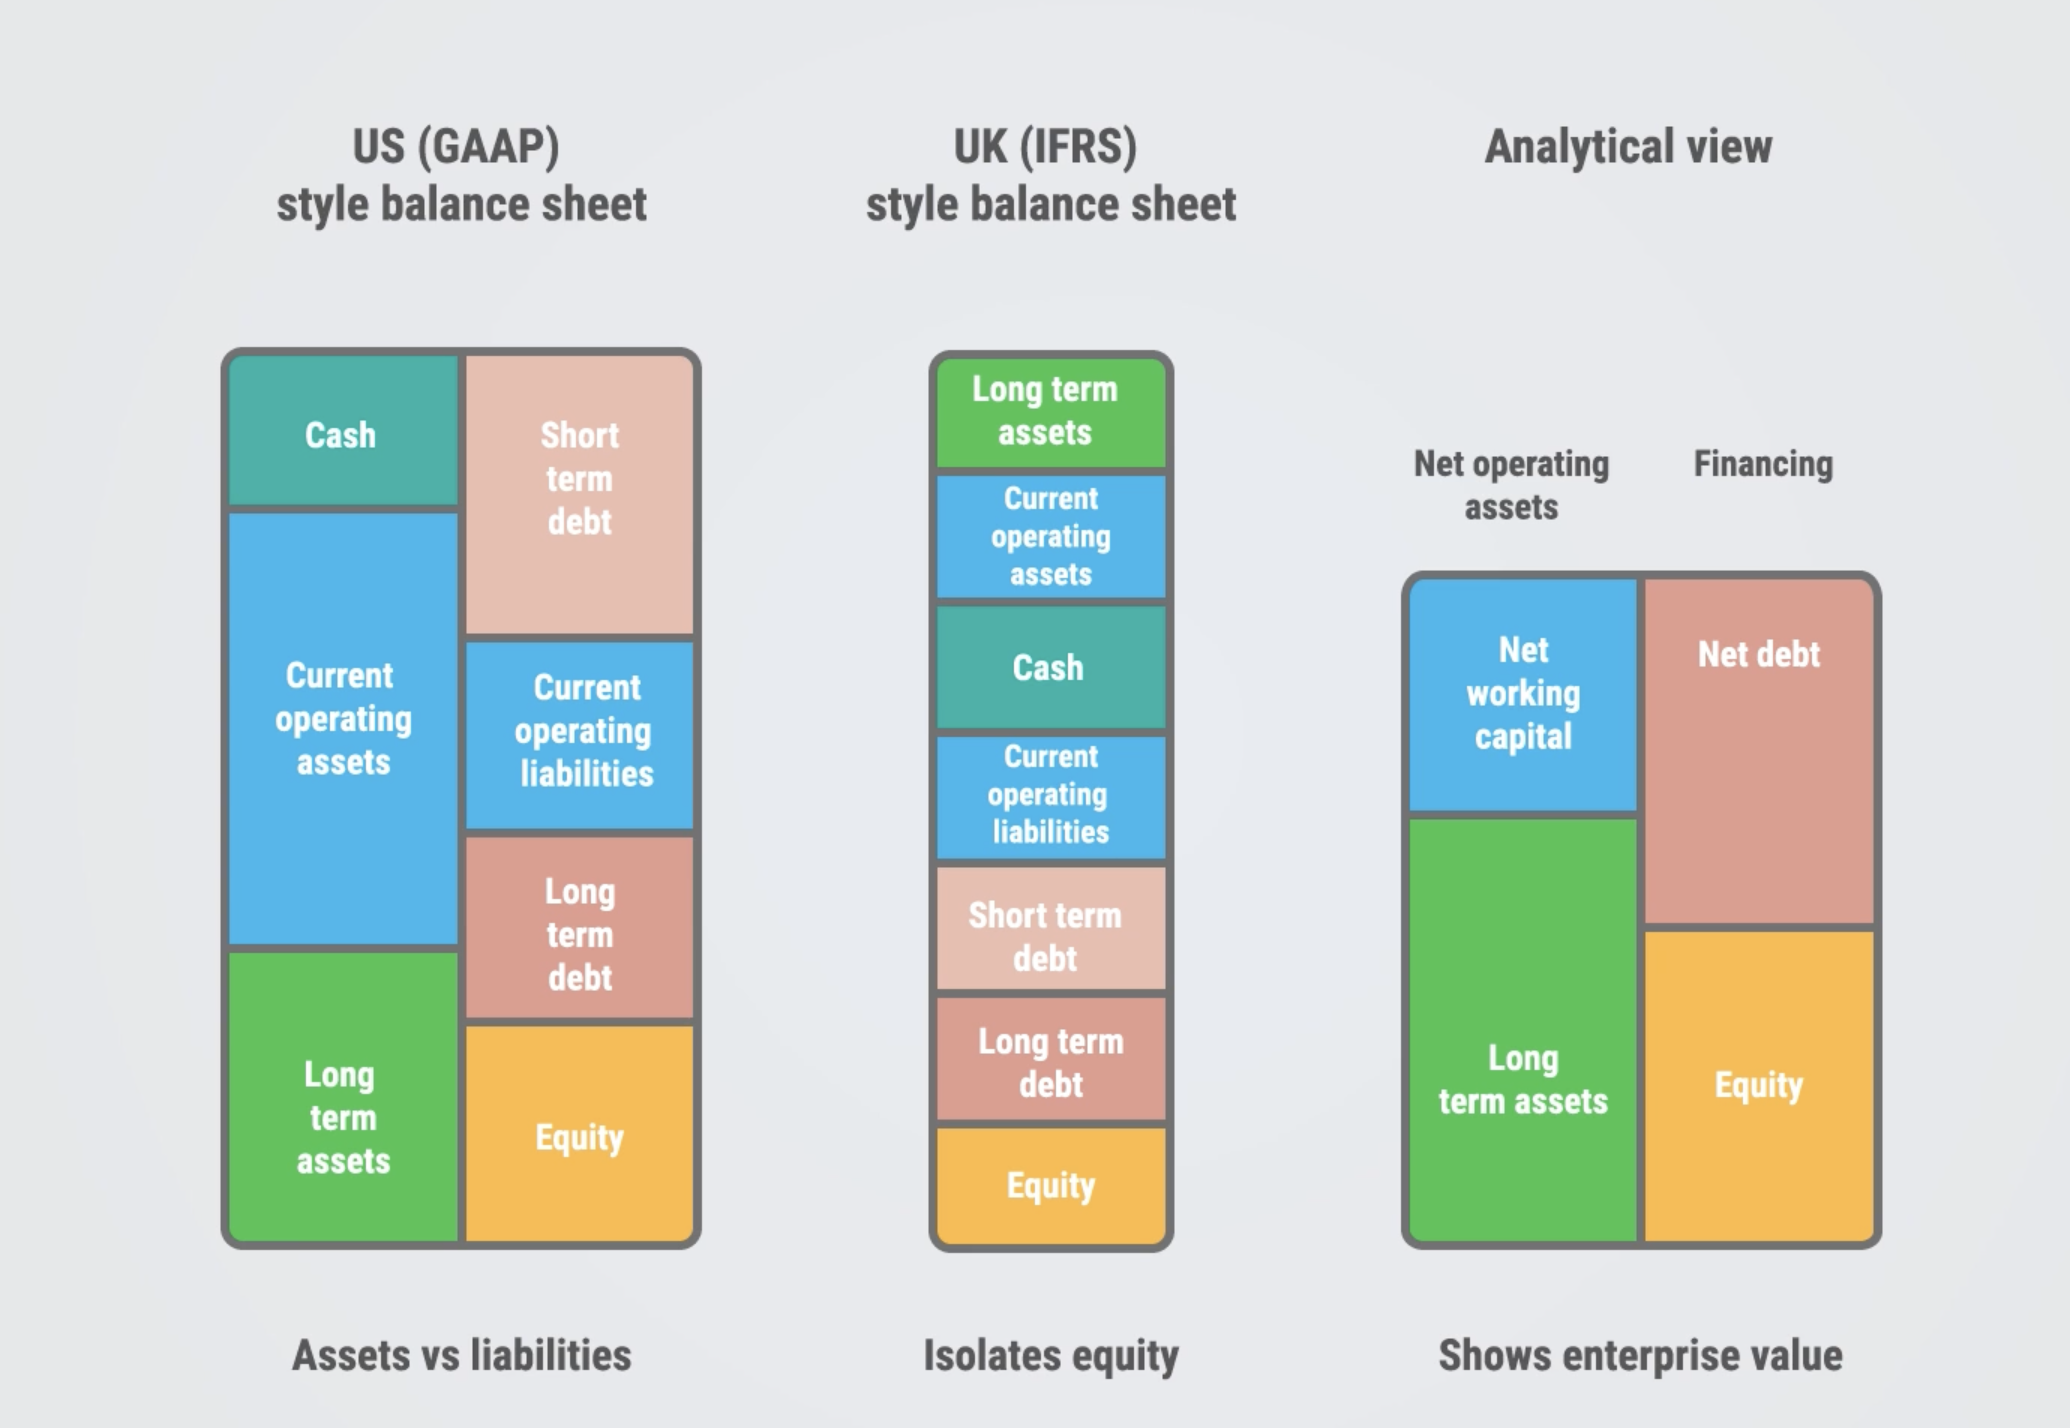
\includegraphics[width=0.8\textwidth]{img/7.3.1.png}
\end{figure}

The balance sheet can be rearranged to show the enterprise value, see Figure \ref{fig:balance_sheet} and Figure \ref{fig:balance_sheet_2}. 

\begin{itemize}
    \item Net working capital
    \item Debt is short-term + long-term debt - cash
    \item Financing of the firm affects cash flows. Debt financing reduces the tax bill, increasing cash flows.
    \item Excessive of debt and the risk of bankruptcy can affect employee and customer behaviour, and suppliers, which could adversely affect cash dlows. 
\end{itemize}

\subsection*{Capital Structure Scenarios}

% \begin{figure}[H]
%     \centering
%     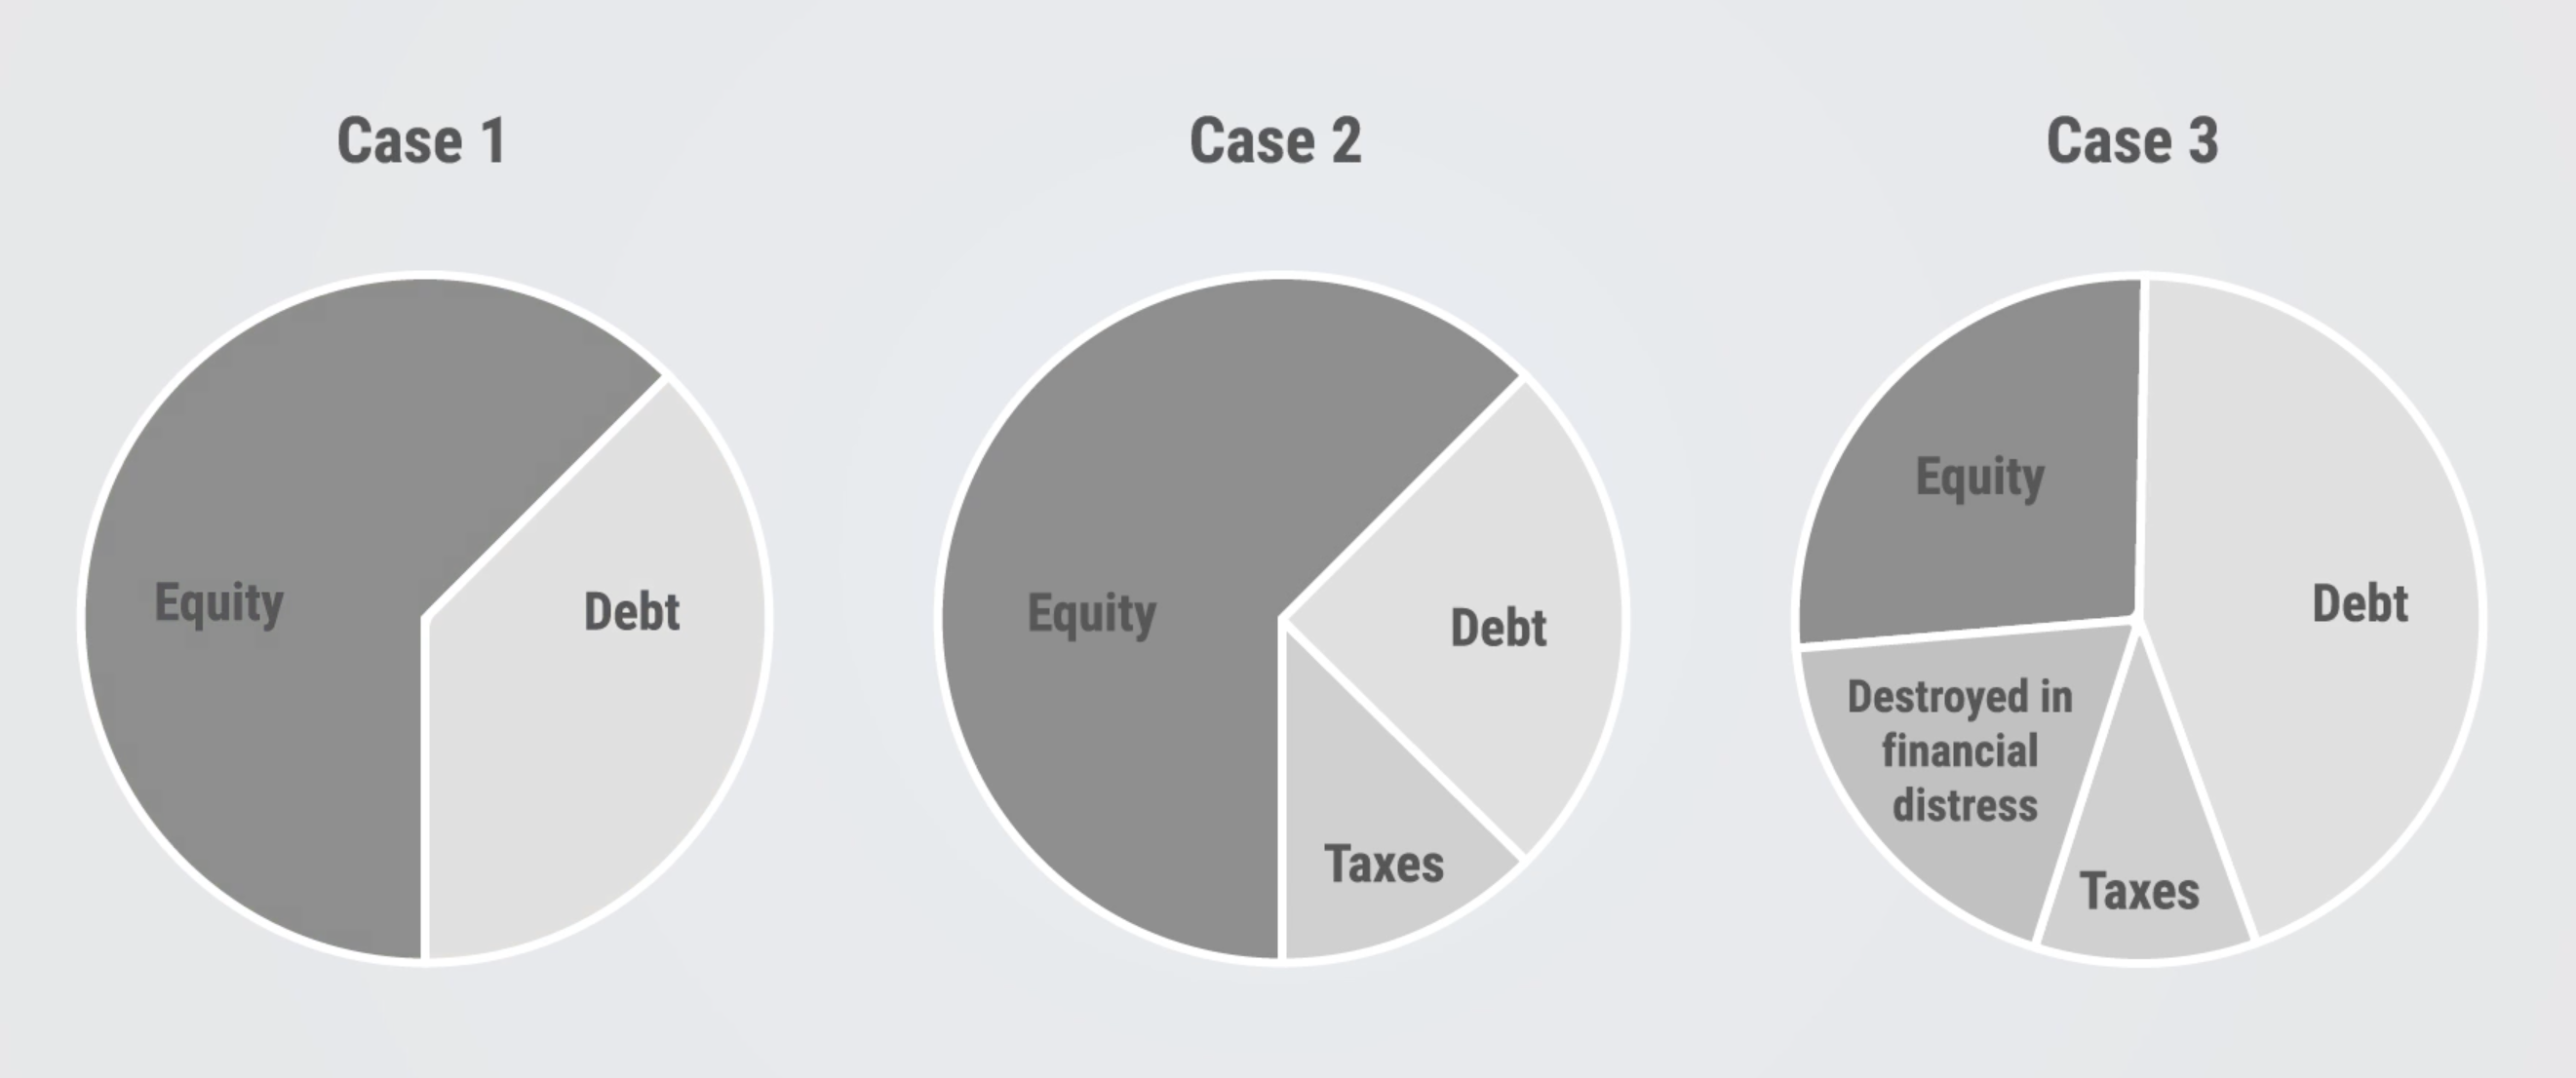
\includegraphics[width=0.8\textwidth]{img/7.3.2.png}
% \end{figure}

\begin{figure}[h]
    \centering
    % Subfigure for Case 1
    \begin{subfigure}{0.3\textwidth}
        \centering
        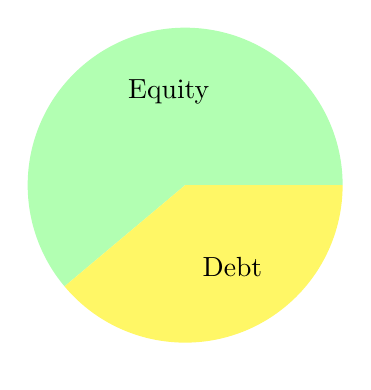
\begin{tikzpicture}
            % Define the slices
            \fill[green!30] (0,0) -- (0:2cm) arc[start angle=0, end angle=220, radius=2cm] -- cycle; % Equity
            \fill[yellow!60] (0,0) -- (220:2cm) arc[start angle=220, end angle=360, radius=2cm] -- cycle; % Debt
            % Labels
            \node at (100:1.2cm) {Equity};
            \node at (300:1.2cm) {Debt};
        \end{tikzpicture}
        \caption{Case 1}
    \end{subfigure}
    % Subfigure for Case 2
    \begin{subfigure}{0.3\textwidth}
        \centering
        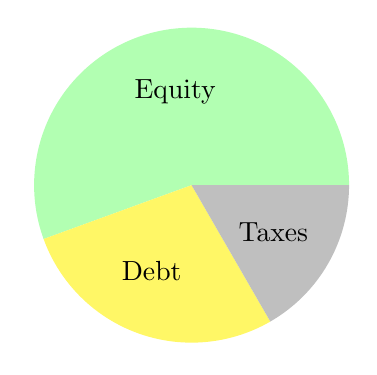
\begin{tikzpicture}
            \fill[green!30] (0,0) -- (0:2cm) arc[start angle=0, end angle=200, radius=2cm] -- cycle; % Equity
            \fill[yellow!60] (0,0) -- (200:2cm) arc[start angle=200, end angle=300, radius=2cm] -- cycle; % Debt
            \fill[gray!50] (0,0) -- (300:2cm) arc[start angle=300, end angle=360, radius=2cm] -- cycle; % Taxes
            % Labels
            \node at (100:1.2cm) {Equity};
            \node at (245:1.2cm) {Debt};
            \node at (330:1.2cm) {Taxes};
        \end{tikzpicture}
        \caption{Case 2}
    \end{subfigure}
    % Subfigure for Case 3
    \begin{subfigure}{0.3\textwidth}
        \centering
        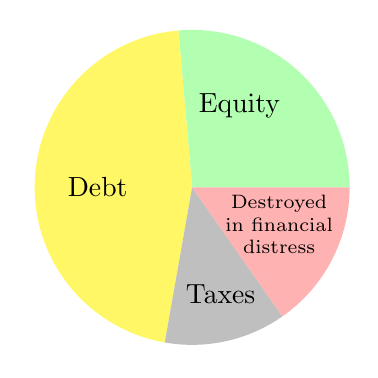
\begin{tikzpicture}
            \fill[green!30] (0,0) -- (0:2cm) arc[start angle=0, end angle=95, radius=2cm] -- cycle; % Equity
            \fill[yellow!60] (0,0) -- (95:2cm) arc[start angle=95, end angle=260, radius=2cm] -- cycle; % Debt
            \fill[gray!50] (0,0) -- (260:2cm) arc[start angle=260, end angle=305, radius=2cm] -- cycle; % Taxes
            \fill[red!30] (0,0) -- (305:2cm) arc[start angle=305, end angle=360, radius=2cm] -- cycle; % Destroyed in financial distress
            % Labels
            \node at (60:1.2cm) {Equity};
            \node at (180:1.2cm) {Debt};
            \node at (285:1.4cm) {Taxes};
            \node[font=\scriptsize, align=center] at (337:1.2cm) {Destroyed \\ in financial \\ distress};

        \end{tikzpicture}
        \caption{Case 3}
    \end{subfigure}
    \caption{Financial composition in three scenarios.}
\end{figure}

\begin{enumerate}
    \item \textbf{Case 1:}
    \begin{itemize}
        \item Perfect capital markets with no taxes or financial distress.
        \item Cash flows are independent of the firm's financing (not affected by financing)
        \item Size of the pie (cash flows) remains constant, financing decisions only affect the size of the slices (cash flows to debt and equity holders)
    \end{itemize}
    \item \textbf{Case 2:}
    \begin{itemize}
        \item Taxes exist in this scenario
        \item Reduces cash paid to investors as some of it goes to the government
    \end{itemize}
    \item \textbf{Case 3:}
    \begin{itemize}
        \item Financial distress costs are present with taxes
        \item Analyse the impact of financial distress on the firm
        \item Size of the pie can decrease due to factors like customer attrition, loss of key employees, reduced credit from suppliers.
        \item This reduces the portion available to debt and equity holders.
    \end{itemize}
\end{enumerate}


\section{Estimating WACC}
This was previously covered in the last chapter's live class.\\

The Weighted Average Cost of Capital (WACC) is the average cost of a company's capital, taking into account the mix of debt and equity used to finance its operations. It is used to discount future cash flows in DCF models to determine the net present value.\\

\begin{equation}
    WACC = \frac{E}{D+E} \cdot r_e + \frac{D}{D+E} \cdot r_d \cdot (1 - \tau_c)
\end{equation}

Where:
\begin{itemize}
    \item $V = E + D$ is the total market value of the firm's financing
    \item $E$ is the market value of equity. $E/V$ is the weight of equity.
    \item $D$ is the market value of debt. $D/V$ is the weight of debt.
    \item $r_e$ is the cost of equity which is required by equity investors. This is estimated using the CAPM model or the Dividend Discount Model (DDM)
    \item $r_d$ is the cost of debt, which can be calculated using the yield to maturity of the firm's existing debt, or considering the interest rate on new debt.
    \item $\tau_c$ is the corporate tax rate. Interest payments on debt are tax-deductible, so $(1 - \tau_c)$ is the tax shield on debt
\end{itemize}

\section{Exercise on Ryanair – Cost of Equity}
Some formulas and a gist of the exercise:
\begin{itemize}
    \item Cost of Equity: $r_e = r_f + \beta \cdot (r_{mkt} - r_f)$ where $r_f$ is the risk-free rate, $\beta$ is the firm's beta, and $r_{mkt}$ is the market return.
    \item Beta can be calculated using the regression of the firm's stock returns against the market returns. 
    \item In Excel, this can be done using the \texttt{lineest(known\_ys, known\_xs, const, stats)} function. Set \texttt{const} and \texttt{stats} to True, and the \texttt{known\_xs} to the excess stock returns, and \texttt{known\_ys} to the market excess returns. The slope of the regression line is the beta.
\end{itemize}

\section{Estimating Debt}
\begin{itemize}
    \item Start by examining the yield to maturity (YTM).
    \item If debt is actively traded, measuring the YTM is straightforward
    \item If debt lacks liquidity or consists of direct loans with the bank, it is more difficult to ascertain market prices and interest rates. Another proxy is needed for the YTM
    \item One proxy approach is to use the company's credit rating or the average credit rating of the debt. 
    \item Another proxy is to use the YTM of debt with a similar rating.
    \item YTM \textbf{assumes no default}, but defaults can occur in practice. 
    \begin{itemize}
        \item To account for this, let the expected return on the debt be the yield to maturity (promised return) minus the expected loss in the event of a default.
        \item The expected loss is calculated as the probability of default multiplied by the loss given a default (LGD).
        \item The probability of default can be estimated from default rates of bonds with similar ratings.
        \begin{equation}
            r_d = YTM - (\text{Probability of Default} \cdot \text{Loss given Default (LGD)})
        \end{equation}
    \end{itemize}
    \item The CAPM and the security market line can also be used to estimate the cost of debt. As corporate bonds tend to be liquid, we can use the debt better of a portfolio of bonds with the same credit rating.
\end{itemize}

\section{Project Valuation}



\begin{itemize}
    \item \textbf{Identify Comparable Companies:} Seek companies specializing in the same products or services. Finding pure play firms can be difficult but focus on those prominently active in the relevant industry.
      \begin{itemize}
        \item \textbf{Pure Play Approach:} Analyse companies within the same industry, e.g., Thomas Cook for package holidays, estimating their betas and adjusting for financial risks.
        \item \textbf{Subjective Approach:} When no perfect match is available, use manual judgement to assess inherent risks. For projects mirroring market average risk, use a beta of 1. If perceived as low-risk, adjust the WACC downward; if high-risk, adjust upward. This approach allows for nuanced consideration of the project's unique characteristics and inherent risks.
      \end{itemize}
    \item \textbf{Estimate Asset Beta:} Determine the asset beta for each identified company. Asset beta (\(\beta_a\)) is calculated using regression analysis and measures the volatility of returns relative to the market.
    \item \textbf{Deleverage Asset Beta:} Convert the asset beta to unlevered beta (\(\beta_u\)) by removing the financial leverage effect, thereby isolating the business risk.
    \begin{equation}
        \beta_u = \frac{\beta_a}{1 + (1 - \tau) \left(\frac{D}{E}\right)}
    \end{equation}
      where \( \tau \) is the tax rate, \( D \) is debt, and \( E \) is equity.
    \item \textbf{Average Unlevered Beta:} Average the unlevered betas of the comparable firms to mitigate individual company variations and better represent the industry’s risk.
    \item \textbf{Adjust for Project Capital Structure:} Modify the averaged unlevered beta to reflect the specific debt-to-equity ratio of the project, thereby tailoring it to the project’s financial structure.
      \begin{equation}
      \beta_{project} = \beta_u \times \left(1 + (1 - \tau) \left(\frac{D}{E}\right)_{project}\right)
\end{equation}
    \item \textbf{Utilise CAPM for Required Return:} Apply the Capital Asset Pricing Model (CAPM) to compute the project's required return:
    \begin{equation}
        r_{required} = r_f + \beta_{project} \times (r_m - r_f)
    \end{equation}
      where \( R_f \) is the risk-free rate, and \( R_m \) is the market return.
  \end{itemize}

  